\cotefile{37}
\scanpage{18}
\margin{\handwritten{\unsure{1.93|1.23}, \unsure{1.27}, 2.9 à reporter au \unsure{3.1}}}

SGA 4 VI

\uline{Sommaire}
\margin{\handwritten{\uline{pp}}}

1. Conditions de finitude pour les objets et flèches d'un topos.\margin{\handwritten{1 à 19}}

2. Conditions de finitude pour un topos.\margin{\handwritten{20 à 37}}

3. Conditions de finitude pour un morphisme de topos. \deleted{\handwritten{\unsure{Cas des limites inductives}}}\margin{\handwritten{38 à 46}}

\deleted{4. Constructibilité.}\inserted{\handwritten{4. Conditions de finitude pour un topos \inserted{obtenu par} recollement.}}\margin{\handwritten{47 à 65}}

\deleted{5}\handwritten{\unsure{6}}. Catégories fibrées et $\underset{\handwritten{\longrightarrow}}{\mathrm{Lim}}$ (rappels).

\deleted{\unsure{6}}\handwritten{7}. Sites et topos fibrés.

\deleted{\unsure{7}}\handwritten{8}. Limites projectives de topos.

\deleted{\unsure{7|8}}\handwritten{\unsure{9|8}}. Cas des limites projectives filtrantes de topos cohérents par morphismes de transition cohérents: théorèmes de passage à la limite pour la cohomologie.
\margin{\handwritten{$\left\{\vphantom{\begin{matrix}a\\b\\c\end{matrix}}\right.$}}

% The curved relocation stroke links the circled replacement number to the position after item 4.
\figure{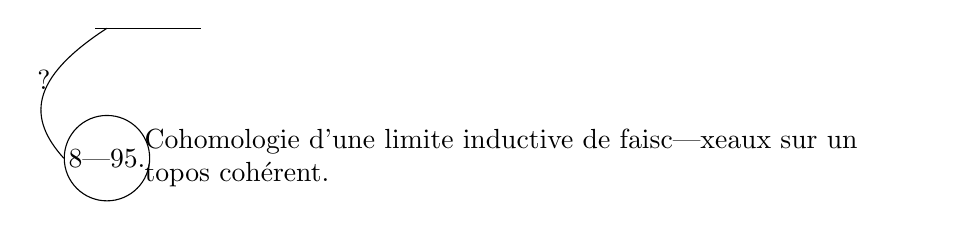
\begin{tikzpicture}[x=0.5cm,y=0.5cm]
\node (a) at (-1.6,2) {\handwritten{\unsure{?}}};
\node[draw,circle,inner sep=1pt] (b) at (0,0) {\deleted{\unsure{8|9}}\handwritten{5}.};
\node[anchor=west,text width=0.82\linewidth,inner sep=2pt] at (0.8,0) {Cohomologie d'une limite inductive de fais\unsure{c|x}eaux sur un topos cohérent\unsure{.}};
\draw (b.west) .. controls (-2,1) and (-2,2) .. (0,3.3);
\draw (-0.3,3.3)--(2.4,3.3);
\end{tikzpicture}}

\handwritten{10. Appendice (par P. Deligne). \deleted{\unsure{Existence de points}} \unsure{d'un|Un} topos cohérent \unsure{a} \inserted{\unsure{suffisamment} de points}.}

\deleted{NB Bien sûr 8 serait interchangeable avec le bloc \deleted{4}\handwritten{5} à \deleted{\unsure{7|8}}\handwritten{\unsure{9}}. Mais il me semble plus naturel de mettre dans deux numéros consécutifs les deux facettes du passage à la limite en cohomologie. Bien sûr, le numéro 8 sera réduit à une ou deux pages, le sorite des conditions de finitude étant déjà fait.}

\deleted{Le n\textsuperscript{o} 4 contiendra le sorite des groupes constructibles (au sens groupes finis ou non), des faisceaux de torsion, des notions de constructibilité pour les Modules et complexes de Modules, - y compris les faits spéciaux dans le cas localement noethérien. Je pense que je le rédigerai mais ne le garantis pas. On peut \deleted{\unsure{à la rigueur}} laisser tomber le n\textsuperscript{o}4, ce sera alors moins beau bien sûr ...:}

\deleted{La rédaction qui suit des n\textsuperscript{o}s 1 à 3 est \unsure{àomplète|complète}, à cela près que je compte y ajouter encore quelques exemples (en particulier un topos localement algébrique non algébrique)\unsure{,|.} \deleted{un morphisme non cohérent de topos cohérents).}}
\inserted{\handwritten{et un topos ayant une famille génératrice formée d'objet\unsure{s} cohérents, qui n'est pas localement algébrique}}
% archive sheet number: 17
\scanpage{23}
\margin{\handwritten{SGA 4 $\overline{\text{\uline{VI}}}$ 2}}

\uline{Exercice} \handwritten{2}. . Soi\inserted{en}t $C$ une \deleted{\unsure{\uline{U}}}\inserted{petite} catégorie\handwritten{,}\inserted{$C'$ une enveloppe de Karoubi\inserted{de $C$ (IV 7.5\handwritten{b))}},} Montrer que les conditions suivantes sont équivalentes:

(i) La catégorie $\mathrm{Ind}(C)$ (I 8.2) est un \uline{$U$}-topos.

( bis) Le foncteur canonique $\mathrm{Ind}(C)\handwritten{\longrightarrow}\overset{\handwritten{\scriptscriptstyle\wedge}}{C}$ admet un adjoint à droite qui \deleted{commute aux} est exact à gauche.

(i ter) Il existe une topologie sur $C$ pour laquelle les faisceaux soient les préfaisceaux ind-représentables.

\deleted{(ii) Dans $C'$, les limites inductives finies sont représentables; \deleted{\unsure{et munissant}}\inserted{il existe sur} $C'$ \deleted{\unsure{d'une}}\inserted{une} topologie dont les familles $(X_i\quad X)_{i\ I}$ sont celles qui sont raffinées par une famille épimorphique finie}

(ii) \deleted{Dans $C'$} Il existe une topologie sur $C'$ dont les familles couvrantes sont celles qui sont raffinées par une famille épimorphique (ou encore, épimorphique effective universelle ..) \uline{finie}, dans $C'$ les limites \deleted{projectives}\inserted{inductives} finies sont représentables, et le foncteur canonique $C\handwritten{\longrightarrow}\overset{\handwritten{\scriptscriptstyle\sim}}{C}$ \deleted{\unsure{est}} y commute.

(iii) (Si dans $C$ les limites projectives finies sont représentables,\deleted{\unsure{à}} de sorte qu'on peut prendre $C'=C$.) Dans $C$ les limites inductives finies sont représentables, et $C$ satisfait la condition ST) de I 8.8 f).
\margin{\handwritten{$\times$}}

(iv) Il existe un topos $\unsure{E|\mathbb{E}}$ engendré par sa sous-catégorie pleine $E_{\mathrm{PF}}$ (\quad\quad), et une équivalence de catégories $C'\handwritten{\approxeq}E_{\mathrm{PF}}$.
\margin{\handwritten{$\times$}}

De plus, \deleted{la topologie} si ces conditions sont satisfaites, la topologie postulée dans (i ter) est nécessairement celle décrite dans (ii), et le topos $E$ postulé dans (iv) est nécessairement équivalent à $\mathrm{Ind}(C)$. Ce topos est donc parfait si et seulement si \inserted{dans} $C'$ \deleted{est} les limites projectives finies sont représentables.
% archive sheet number: 22
\scanpage{24}
% letterhead
\begin{center}
I N S T I T U T\\
DES HAUTES ÉTUDES SCIENTIFIQUES\\
\rule{1cm}{0.4pt}
\end{center}

\handwritten{SGA 4 $\overline{\text{\uline{\unsure{VII|VI}}}}$\quad p. 20}

\handwritten{\uline{Ajouter} 5.6. \textcircled{a} $\tilde{X}_{\mathrm{et}}$ est \inserted{algébrique\inserted{(ref)}, \unsure{d.|de} torsion,} localement cohérent\inserted{(ref)}. Il est cohérent \deleted{\illegible{1}}\inserted{(ref)} (\unsure{resp.} quasi-séparé\inserted{(ref)}) \deleted{\illegible{1}} \unsure{sss|ssi} le schéma $X$ est \deleted{\unsure{quasi-cpt}} cohérent i.e. qu. cpt qu. sép (resp. quasi-séparé). \deleted{\illegible{1}}}

\handwritten{\textcircled{b} Soit $(X_i)_{i\in I}$ système projectif filtrant à morphismes de transition affines, $X=\varprojlim_i X_i$ (EGA \uline{IV} 8);}

\handwritten{\unsure{Âlors|Alors}}
\[
\handwritten{\tilde{X}_{\mathrm{et}}\simeq\underset{\longleftarrow}{\mathrm{limtop}}\,\tilde{X}_i.}
\]

\handwritten{En déduire pour 5.7.}

\margin{\handwritten{\uline{Cor.} 5.6.1. $X'\in\mathrm{Ob}\,\unsure{X_{\mathrm{et}}|\tilde{X}_{\mathrm{et}}}$ est \deleted{\unsure{cohérent}} \inserted{\textcircled{\scriptsize\unsure{qu.-cpt}}} (\unsure{qu. sép}) dans $X_{\mathrm{et}}$ sss $X'$ est \deleted{\illegible{1}}. \inserted{\textcircled{\scriptsize\unsure{resp. coh}}}}}
\figure{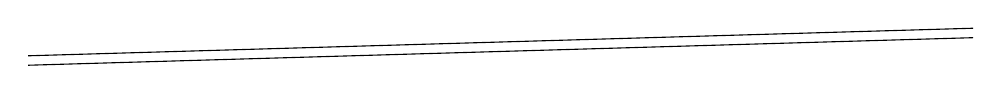
\begin{tikzpicture}\draw (0,0)--(12,0.35);\draw (0,-0.12)--(12,0.23);\end{tikzpicture}}

\handwritten{SGA 4 $\overline{\text{\uline{IX}}}$\quad p. 42\qquad note \uline{pour} la p. 8}
\figure{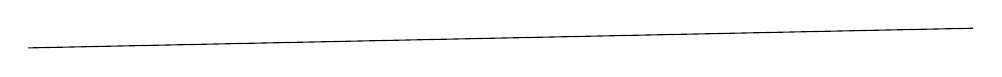
\begin{tikzpicture}\draw (0,0)--(12,0.25);\end{tikzpicture}}

\handwritten{$\overline{\text{\uline{VII}}}$\quad 2.1 c)\qquad (p. 9)\quad \uline{corriger}}
% archive sheet number: 23
\scanpage{25}
\handwritten{SGA 4 \uline{IX}\quad p. 42}
\margin{\handwritten{nous prouverons en même temps que $\tilde{X}_{\mathrm{et}}$ satisfait aux conditions équivalentes de \uline{VI} 1.2\unsure{).|].}}}

\handwritten{(*) (Note pour la page 8.) Prouvons que la notion de constructibilité 2.3 pour un faisceau d'ensembles $F$ coïncide avec celle de \uline{VI} 1.9.3. \deleted{Soit} La \deleted{\unsure{en effet $C$ le cas}}\inserted{question étant} locale sur $X$, on peut supposer $X$ affine \inserted{donc ``cohérent'', i.e.} quasi-compact et quasi-séparé. \deleted{Soit $C$ la catégorie \unsure{Soit $(C')$ le sous}\illegible{1}} \deleted{\unsure{Il|Je} faut alors prouver que $F$ est constructible} Soit $C$ (resp. $C'$) la sous-catégorie \deleted{\unsure{pleine}}\inserted{strictement} pleine de $\tilde{X}_{\mathrm{et}}$ formée des $F$ constructibles au sens de 2.3, \deleted{\illegible{1}} \inserted{(resp. au sens de \uline{VI} 1.9.3), il} faut prouver \deleted{que $C$ s'identifie à la catégorie des objets \uline{cohérents} de} \deleted{\unsure{$\tilde{X}_{\mathrm{et}}$}} que $C=C'$;}

\handwritten{\deleted{En vertu de \uline{VII} 5.6 a), \deleted{l'objet final $X$ de} $\tilde{X}_{\mathrm{et}}$ \deleted{est cohérent, donc} $C'$ est formé des objets \uline{cohérents} \deleted{\unsure{\uline{VI}}} de $\tilde{X}_{\mathrm{et}}$ (2.5). En vertu de \uline{VI} 1.24, \deleted{\unsure{et}} et compte tenu du fait que $C$ est génératrice dans $\tilde{X}_{\mathrm{et}}$ (2.7.2) et stable par limites inductives finies (2.\unsure{6|8} (i)), il suffit de prouver que $C\subset C'$, Mais il résulte de 2.7 que tout $F\in\mathrm{ob}\,C$ est \uline{quasi-compact}, puisque un \deleted{\unsure{$G\in\mathrm{ob}\,X_{\mathrm{et}}$}}\inserted{$\unsure{G|C}\in X'_{\mathrm{et}}$} \deleted{\unsure{schéma $X'$}} qui est quasi-compact et quasi-séparé est quasi-compact comme objet de $\tilde{X}_{\mathrm{et}}$ \deleted{(5.6.1)} (\uline{VII} 5.6.1). \deleted{D'autre part pour \unsure{voir que} $\unsure{F|F'}\unsure{\in|\to}\unsure{\mathrm{ob}\,X'|X'}$ la diagonale $F\longrightarrow F\mathbin{\times}_{X}F$ est quasi-compacte, il suffit de voir que \unsure{pour tout} \illegible{2} \unsure{et que}\illegible{2} \unsure{ce fait que $C$ est stable par produits}} Comme $C$ est stable par \deleted{limites projectives}\inserted{produits} finis\inserted{(2.6 (ii))}, l'inclusion $C\subset C'$ est donc un cas particulier de 2.1.}}
\margin{\handwritten{\deleted{\unsure{pourquoi|pour} \unsure{préciser}}}}

\handwritten{En vertu de \uline{VI} 2.9, b), il suffit de voir que $C$ est stable pour limites inductives finies et limites projectives finies, qu'elle est génératrice, et formée d'objets quasi-compacts. \deleted{\illegible{1}} Compte tenu de 2.6 (i) et (2.7.2), il reste à prouver que tout $F\in\mathrm{ob}\,C$ est quasi-compact. Or \deleted{cela résulte}\inserted{en vertu} de 2.7 \deleted{\unsure{et} \uline{VI} 1.3}, \deleted{puisque}\inserted{il existe} un $G\in\mathrm{ob}\,X_{\mathrm{et}}$ \deleted{\illegible{1}} qui est \inserted{un schéma} quasi-compact et quasi-séparé \deleted{\unsure{et est}} et un épimorphisme $G\longrightarrow F$. Or $G$ \deleted{\unsure{comme on}} est un objet quasi-compact de $\tilde{X}_{\mathrm{et}}$ (\uline{VII} 5.6.1), donc $F$ est quasi-compact (\uline{VI} 1.3), qfd.}

\handwritten{Bien entendu, il y aurait \inserted{eu} lieu de refondre les §§ 1,2 du présent exposé, \inserted{notamment} en les rattachant \deleted{\unsure{explicitement}} aux notions générales de \deleted{l'exposé} finitude de \uline{VI}. Nous laissons ce soin \deleted{\unsure{complémentaire}} de rédaction aux générations futures.}
% archive sheet number: 24
\scanpage{27}
\mspage{\handwritten{19}}
% The source is upside down; read after a 180-degree rotation.
% The entire draft is cancelled by long diagonal strokes.
\margin{\handwritten{\textcircled{$\unsure{\psi|\Psi}$}}}

\deleted{2.1.1. On peut dire encore qu'une structure de biextension sur le $G_{P\times Q}$-torseur $E$ est définie par deux lois de composition non partout définies $\handwritten{\phi}(x,y)$ et $\handwritten{\unsure{\mu|\psi}}(x,y)$ sur $E$, la première étant définie lorsque \deleted{\unsure{$j($}} $\mathrm{pr}_2j(x)=\mathrm{pr}_2j(y)$, la deuxième lorsque $\mathrm{pr}_1j(x)=\mathrm{pr}_1j(y)$ \deleted{(où} (où $j:E\handwritten{\longrightarrow}P\times Q$ est le morphisme structural du torseur). Les axiomes, en plus des associativités du type}
\[
\deleted{\deleted{\handwritten{\phi}(gx,y)\unsure{=}g\handwritten{\phi}(x,y)\unsure{,}\quad\handwritten{\phi}(x,gy)\unsure{=}g\handwritten{\phi}(x,y)\quad\handwritten{\phi}(}}
\]
\[
\deleted{\handwritten{\phi}(gx,y)=\handwritten{\phi}(x,gy)=g\handwritten{\phi}(x,y)\qquad(x,y\handwritten{\in}E(S),\ g\handwritten{\in}G(S))}
\tag*{(2.1.1.1)}
\]

\deleted{et des relations analogues en $\handwritten{\mu}$, s'expriment alors par l\deleted{a}'associativité et la commutativité de \unsure{ces|ses} lois de composition partielles, et par la relation}
\[
\deleted{\handwritten{\phi}(\handwritten{\mu}(x,y),\handwritten{\mu}(z,t))=\handwritten{\mu}(\handwritten{\phi}(x,z),\handwritten{\phi}(y,t))}
\tag*{(2.1.1.2)}
\]
\deleted{pour $x,y,z,t$ respectivement dans $E_{p,q}(S),E_{p,q'}(S),E_{p',q}(S),E_{p',q'}(S)$.}

\deleted{2.2. \inserted{\handwritten{\uline{Sections unité}.}} Il y a lieu de considérer la section unité de $\mathbb{E}\deleted{\unsure{t|E}}$ considéré comme extension de $Q_P$ par $G_P$,}
\[
\deleted{e_{E/P}\handwritten{\in\Gamma}(E/P)=\mathrm{Hom}_P(P,E)\ ,}
\tag*{(2.2.1)}
\]
\deleted{et de façon symétrique la section unité de $E$ considéré comme extension de $P_Q$ par $G_Q$,}
\[
\deleted{e_{E/Q}\handwritten{\in\Gamma}(E/Q)=\mathrm{Hom}_Q(Q,E)\ .}
\tag*{(2.2.2)}
\]

\deleted{En particulier, \uline{le torseur} $E$ \uline{au dessus de} $P\times Q$ (de \unsure{G|g}roupe $G_{P\times Q}$) \uline{est canoniquement trivialisé au dessus de} $1_P\times Q$ \uline{par} $e_{E/P}$, \uline{et au dessus de} $P\times1_Q$ \uline{par} $e_{E/Q}$. \inserted{De plus,} \uline{Ces deux trivialisations coïncident au dessus de la section unité} $1_P\times1_Q$ de $P\times Q$, et définissent\inserted{\handwritten{donc}} une même section}
\[
\deleted{e_{E\deleted{\unsure{/S|/P|/Q}}}\handwritten{\in\Gamma}(E\handwritten{)}\deleted{\unsure{/S)|/P)|/Q)}}\ ,}
\tag*{(2.2.3)}
\]
\deleted{qu'on appellera par abus de langage la \uline{section unité} (ou \uline{section neutre}) de $E$. Pour prouver l'égalité annoncée\deleted{\unsure{et une conséquence}} des deux sections $e,e'$ de $E$ déduites respectivement de $e_{E/P}$ et $e_{E/Q}$, on note}
% archive sheet number: 26
\scanpage{30}
\margin{\handwritten{SGA 4 $\overline{\text{\uline{XVI}}}$}}
\mspage{VII 2}

Du point de vue substance, 2.1.1 se ramène trivialement au cas où dans $X\handwritten{\longrightarrow}S$, $X$ est affine, donc quasi-compact quasi-séparé (on dit maintenant ``cohérent''), et alors c'est une conséquence du th. de changement de base par $f$, qui est donné dans SGA 4 XVI 1.1\inserted{et qui est essentiellement}. Mais dans loc. cit. on utilise toute la force du théorème de changement de base propre, ce qui est en effet abusif, car en interprétant comme un énoncé d'acyclicité globale 2.1.1, on est ramené comme tu l'observes \deleted{à 2.1.5} au cas particulier 2.1.5, qui se ramène trivialement à son tour au cas du degré de transcendance 1, et par là au th. de changement de\inserted{corps de} base pour le $H^1$ premier à $p$ pour une courbe propre et lisse. Je pense présenter les choses ainsi en réédition de SGA 4, de sorte que ton 2.1.1 y sera énoncé en toutes lettres, s'il ne l'est déjà (je n'ai pas les textes en main). Cela te dispensera donc de le prouver, ta seule tâche consistant à interpréter en termes de champs cet énoncé \deleted{(que tu pourrais donner sous forme de rappels)}.
\margin{\figure{\begin{tikzpicture}\draw (0,0) .. controls (.45,-.12) and (.60,-.15) .. (1.1,.5);\end{tikzpicture}}}

Du point de vue rédaction, on a l'impression que tu t'es ingénié à tout présenter à l'\unsure{e|E}nvers. Il faut en tous cas bloquer ensemble 2.1.1 et 2.1.7 (pratiquement identiques) et 2.1.5 (celui-ci en corollaire, peut-être) \deleted{- ce sera dans les rappels}\inserted{\handwritten{cf texte joint}}\deleted{. Avant même de donner ces énoncés, il faudra avoir rappelé les définitions, pour que ça ait un sens.} \deleted{Au lieu de pro-lisse resp. lisse, il suffit\inserted{dans le tH.} de supposer tout \uline{localement} \uline{$L$-\inserted{\unsure{1-|l-}}asphérique} (``par exemple ...'' ).} D'autre part, \deleted{les énoncés} 2.12, 2.1.3, 2.1.4, 2.1.7.1 n'ont rien à voir avec les schémas, il sont manifestement importants en eux-mêmes et devraient passer dans un numéro à part dans \handwritten{\uline{IV}\deleted{\unsure{6|5}}\inserted{ou \uline{V}}} (avec un peu d'ordre dans la suite des énoncés)
\margin{\handwritten{\unsure{si on utilise} \unsure{ailleurs} la ``factorisation canonique d'un champ'',}}

\deleted{Enfin, les compléments schématiques 2.1.7.2 à 2.1.7.4 \unsure{de|d}}
% archive sheet number: 29
\scanpage{31}
\margin{\figure{\begin{tikzpicture}\draw (0,0) -- (0,-6);\end{tikzpicture}}}
\uline{Théorème} 2.1.1. Soit $f:S'\handwritten{\longrightarrow}S$ un morphisme universellement localement \uline{$L$}-\unsure{1|l}-asphérique (SGA 4 XV \handwritten{1.11}), par exemple (SGA\handwritten{4}XV \handwritten{2.2}) un morphisme lisse, ou tel que $\unsure{S|\mathbb{S}}\handwritten{'}$ soit isomorphe à la limite\inserted{projective} d'un systême projectif\inserted{filtrant} de $S$-schémas lisses $S'_i$ à morphismes de transition affines\deleted{\unsure{,}} (SGA 4 XV \handwritten{1.13\inserted{(ii)}})

Soi\inserted{en}t $g:X\handwritten{\longrightarrow}S$ un morphisme de schémas, d'où un carré car\deleted{\unsure{ét|té}}\unsure{té|ét}sien
\diagram{\begin{tikzcd}[ampersand replacement=\&]
X \handwritten{\arrow[d,"g"']} \& X' \handwritten{\arrow[l,"f'"']} \handwritten{\arrow[d,"g'"]} \\
S \& S'\handwritten{\arrow[l,"f"']}\rlap{,}
\end{tikzcd}}

$G$ un\inserted{ind-\uline{$L$}-} champ sur $X$ \deleted{dont les faisceaux d'automorphismes sont des ind-\uline{$L$}-faisceaux}\inserted{(\uline{V} \handwritten{5}\quad)}, $G'=f'^*(G)$ le champ image inverse sur $X'$.

\begin{enumerate}[label=\alph*)]
\item Si \deleted{$S$ et $S'$ sont strictement locaux et} $f$ est un morphisme \deleted{strictement} \uline{local} de schémas strictement locaux, alors le foncteur
\[
\handwritten{G(X)\longrightarrow G'(X')}
\]
est une équivalence de catégories.

\item Si $g$ est cohérent(i.e. quasi-compact et quasi-séparé) alors le morphisme de champs ``de changement de base''
\[
f^{\handwritten{'}}(g_{\handwritten{*}}(G))\handwritten{\longrightarrow}g'_{\handwritten{*}}(f'^{\handwritten{*}}(G))\deleted{\handwritten{\unsure{=g_*|g_*}}}
\]
est une équivalence de champs sur $S'$.
\end{enumerate}

\margin{\figure{\begin{tikzpicture}\draw (0,0) -- (0,-2);\end{tikzpicture}}}
\uline{Corollaire} 2.1.2. Soient $k$ un corps séparablement clos, $k'$ une extension séparablement close de $k$, $X$ un $k$-schéma, $X'=X\handwritten{\otimes}_k k'$, alors pour tout \deleted{champ $G$} ind-\uline{$L$}-champ $G$ sur $X$, désignant par $G'$ son image inverse sur $X'$, le foncteur
\[
\handwritten{G(X)\longrightarrow G'(X')}
\]
est une équivalence de catégories.

O\unsure{n|p} sait en effet (SGA 4 XVI\quad\quad) que $\operatorname{Spec}(k')\handwritten{\longrightarrow}\operatorname{Spec}(k)$ est universellement localement \uline{$L$}-1-asphérique.

Démonstration. On prouve a) par référence à SGA 4 XVI (nouvelle édition !),\inserted{\handwritten{et à \uline{V} --}} et b) en se ramenant à a) par des lemmes 2.1.7.2 et 2.1.7.4 renumérotés.
\margin{\handwritten{En tout, ça devrait faire 3 pages au \unsure{Ch.p|Chap.|Ch.} $\overline{\text{\uline{VII}}}$ au maximum, -- mais il y aurait renvois au Ch.p $\overline{\text{\uline{V}}}$.}}
% archive sheet number: 30
\scanpage{34}
\unsure{\deleted{exp XIII 3.1: You wrote that proof, so if you think one needs the noetherian assumption, I agree.}}

\figure{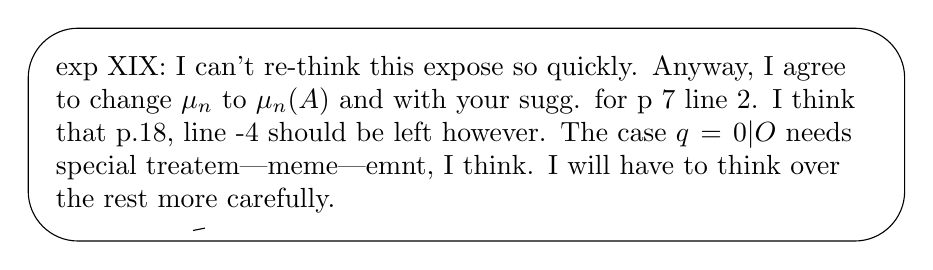
\begin{tikzpicture}
\node[draw,rounded corners=18pt,inner sep=10pt,text width=0.86\linewidth] (note) {exp XIX: I can't re-think this expose so quickly. Anyway, I agree to change $\handwritten{\mu}_n$ to $\handwritten{\mu}_n(A)$ and with your sugg. for p \handwritten{7} line \handwritten{2}. I think that p.18, line \handwritten{-4} should be left however. The case $q=\unsure{0|O}$ needs special treat\deleted{\unsure{em|me}}\unsure{me|em}nt, I think. I will have to think over the rest more carefully.};
\draw ([xshift=2.1cm,yshift=4pt]note.south west)--++(0.15,0.03);
\end{tikzpicture}}
% stamp: faint circular institutional seal showing through the sheet; wording not reliably legible.
% archive sheet number: 33
\scanpage{35}
% Long diagonal strokes cancel this sheet.
\deleted{reference [1] for expose X :}

\deleted{[1] J. Ax , Some conjectures of Serre on cohomological dime\deleted{\unsure{s|a|n}}nsion, Proc. Amer. Math. Soc. 16 (1965) 1214-1221 .}
\figure{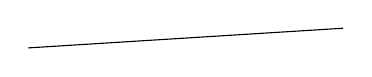
\begin{tikzpicture}\draw (0,0)--(4,0.25);\end{tikzpicture}}

\deleted{exp X p. 7 here is what is to be added:}

\deleted{Le corps residuel de $R'$ est $k$ puisque nous avons suppose $\bar{G}$ un \deleted{$\unsure{p|m}$} $\handwritten{\ell}$-groups, donc que les racines $\handwritten{\ell}$-iemes de 1 so\deleted{\unsure{t|n}}nt dans $K$. On a un diagramme}
\diagram{\begin{tikzcd}[ampersand replacement=\&]
\deleted{H'} \handwritten{\arrow[r,hook]}\handwritten{\arrow[d,hook]} \& \deleted{G'} \handwritten{\arrow[r]}\handwritten{\arrow[d,hook]} \& \deleted{\bar{G}} \handwritten{\arrow[d,equal]} \\
\deleted{H} \handwritten{\arrow[r,hook]} \& \deleted{G} \handwritten{\arrow[r]} \& \deleted{\bar{G}}\rlap{,}
\end{tikzcd}}
\figure{\begin{tikzpicture}\draw (0,0)--(3.2,0);\end{tikzpicture}}

\deleted{exp XII, 5.10: A reference for my paper on alg.approx is}

\deleted{M. Artin, Algebraic approximation of structures over complete local rings, (a paraitre).}

\deleted{\handwritten{(}The explicit result is Theorem (3.1)\handwritten{)}.}
\figure{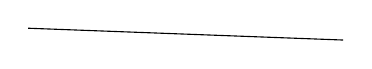
\begin{tikzpicture}\draw (0,0)--(4,-0.15);\end{tikzpicture}}

\deleted{exp IX p.\handwritten{34} here are some references:}

\deleted{A. Douady, Cohomologie des groupes compacts totalement discontinus, Séminaire Bourbaki, exposé 189, (th\handwritten{\unsure{ê|é}}or\handwritten{è}me 4.3)}

\deleted{S. Lang, Rapport sur la cohomologies des groupes, Benjamin 1966. (th\handwritten{é}or\handwritten{è}me 12, p.207).}

\deleted{Ch.C. Tsen, Divisionsalgebren über Funktionen\deleted{\unsure{f|k}}körper, Nachr. Ges. Wiss. Göttingen (1933) \handwritten{335-339} .}
% archive sheet number: 34
